\subsection{ERM and DRO have poor worst-group accuracy in the overparameterized regime}\label{sec:experiments_unreg}

Overparameterized neural networks can perfectly fit the training data and still generalize well on average \citep{zhang2017understanding}.
We start by showing that these overparameterized models do not generalize well on the worst-case group when they are trained to convergence using standard regularization and hyperparameter settings \citep{he2016resnet, devlin2019bert}, regardless of whether they are trained with ERM or group DRO.\footnote{
  Training to convergence is a widespread practice for image models \citep{zhang2017understanding, hoffer2017train}. Pre-trained language models are typically pretrained until convergence \citep{devlin2019bert, radford2019language} but fine-tuned for a fixed small number of epochs because average test accuracy levels off quickly; we verified that training to convergence gave equally high average test accuracy.}

\paragraph{ERM.}
As expected,
ERM models attain near-perfect worst-group training accuracies of at least $99.9\%$ on all three datasets
and also obtain high average test accuracies ($97.3\%$, $94.8\%$, and $82.5\%$ on Waterbirds, CelebA, and MultiNLI).
However, they perform poorly on the worst-case group at test time
with worst-group accuracies of $60.0\%$, $41.1\%$, and $65.7\%$ respectively (\reftab{analysis}, \reffig{train}).
Their low worst-group accuracies imply that these models are
brittle under group shifts.

\paragraph{DRO.}
The ERM models trained above nearly perfectly classify every training point, and are therefore near-optimal for both the ERM \refeqn{hterm} and DRO \refeqn{htdro} objectives.
Indeed, we find that group DRO models perform similarly to ERM models,
attaining near-perfect training accuracies and high average test accuracies, but poor worst-group test accuracies (\reftab{analysis}, \reffig{train}).

\paragraph{Discussion.}
The ERM and DRO models attain near-perfect training accuracy and vanishing training loss
even in the presence of default regularization (batch normalization and standard $\Ltwo$ penalties for ResNet50, and dropout for BERT).
However, despite generalizing well on average, they do \emph{not} generalize well on the worst-case group, and consequently suffer from low worst-group accuracies.
This gap between average and worst-group test accuracies arises not from poor worst-group training performance---the models are near-perfect at training time, even on the worst-case groups---but from variations in the generalization gaps across groups. Even though DRO is designed to improve worst-group performance, we find no improvements on worst-group test accuracies since the models already achieve vanishing worst-group losses on the \emph{training} data.

\begin{table}[!t]
  \vspace{-6mm}
  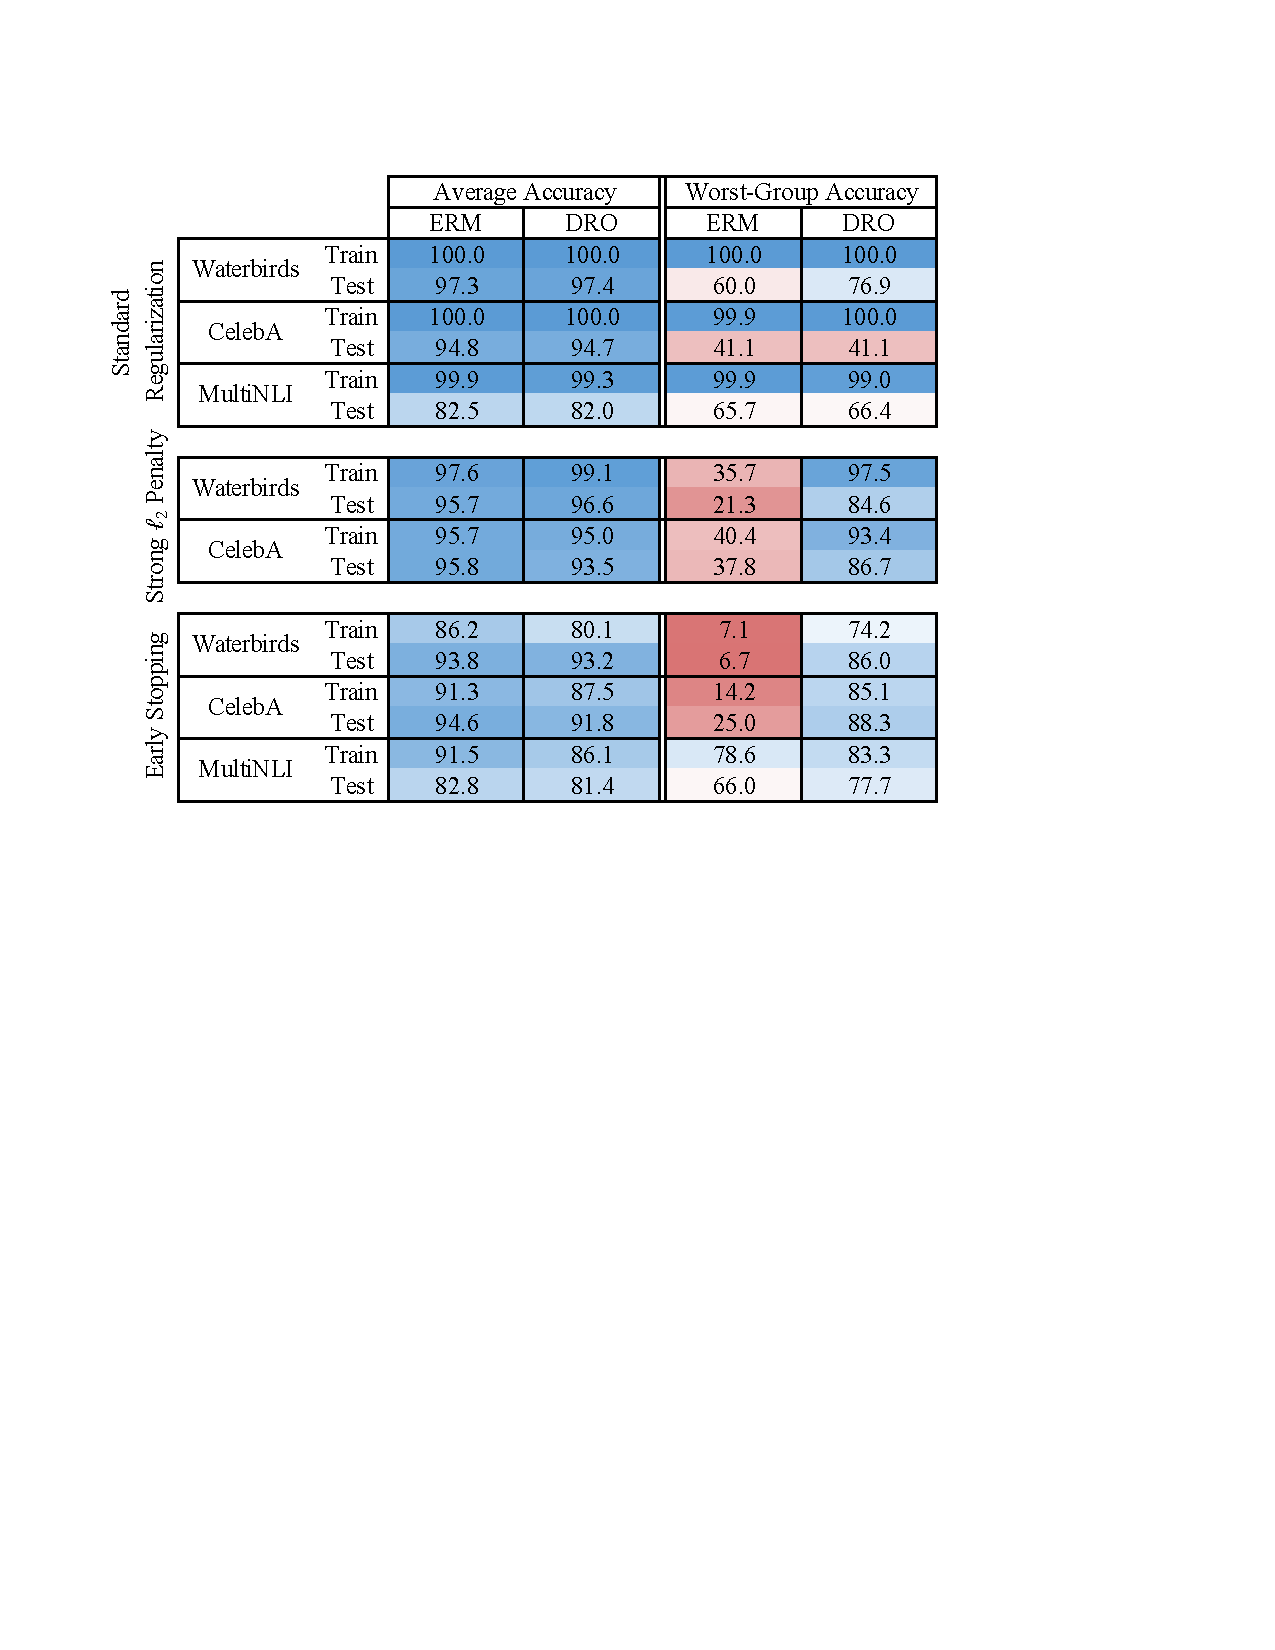
\includegraphics[width=0.8\textwidth]{figs/table_1.pdf}
  \centering
  \caption{
  Average and worst-group accuracies for each training method. Both ERM and DRO models perform poorly on the worst-case group in the absence of regularization (top). With strong regularization (middle, bottom), DRO achieves high worst-group performance, significantly improving from ERM. Cells are colored by accuracy, from low (red) to medium (white) to high (blue) accuracy.
    }
  \label{tab:analysis}
\end{table}

\begin{figure}[!t]
\centering
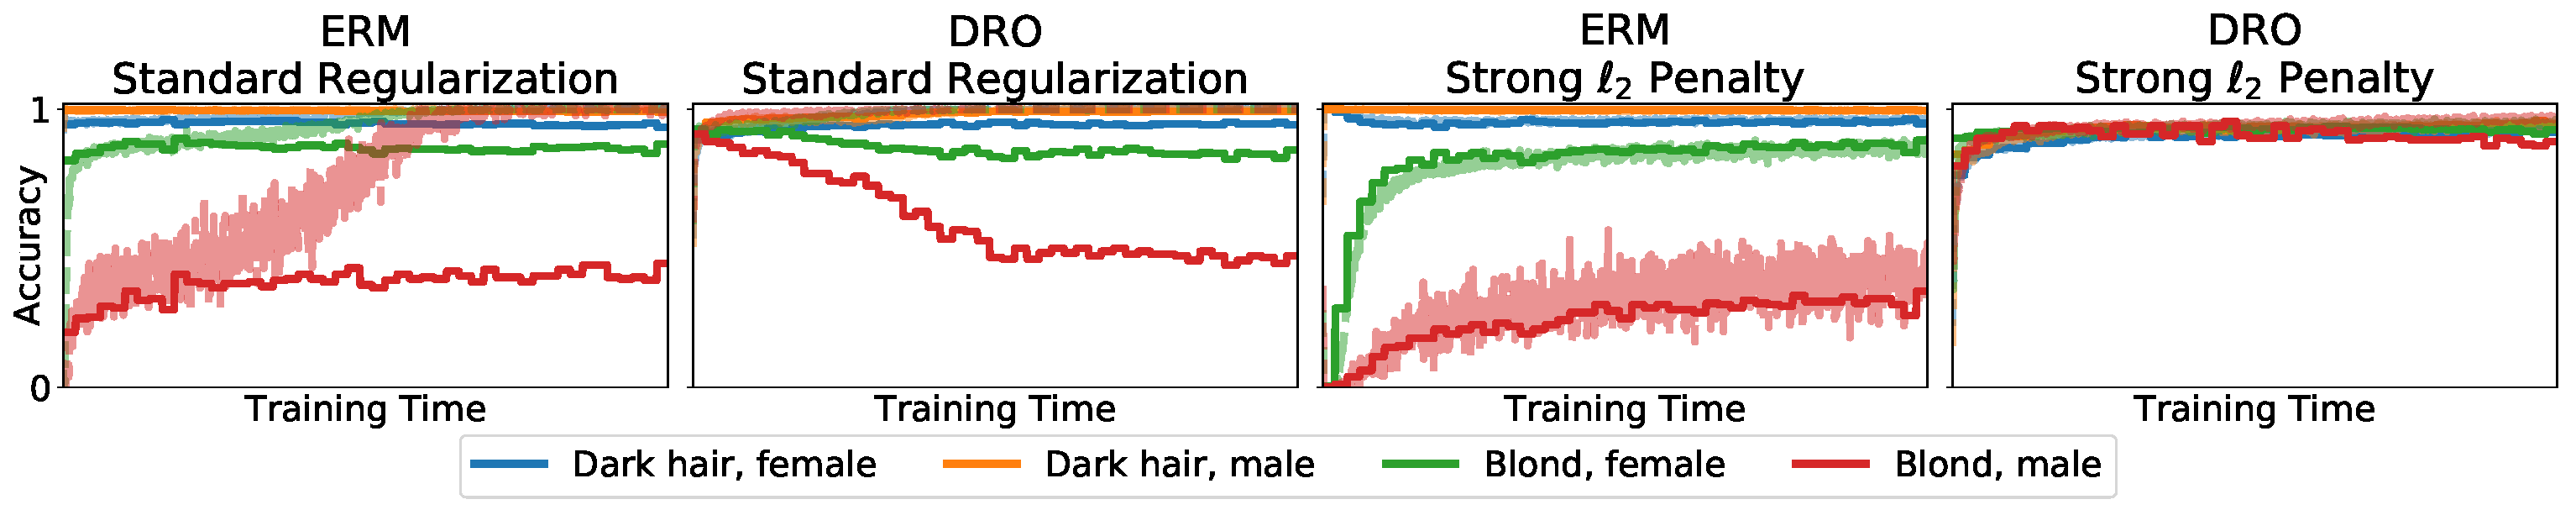
\includegraphics[width=\textwidth]{figs/train_curve.pdf}
  \caption{Training (light) and validation (dark) accuracy for CelebA throughout training. With default hyperparameters and training to convergence, ERM and DRO models achieve perfect training accuracy across groups, but generalize badly on the worst-case group (red line in the left panels). With strong $\Ltwo$ penalties, ERM models get high average train and test accuracies at the cost of the rare group (panel 3). DRO models achieve high train and test accuracies across groups (panel 4).
  }
  \label{fig:train}
\end{figure}
